\documentclass{article}

\usepackage[margin=1in]{geometry}
\usepackage{amsmath}  
\usepackage{graphicx} 
\usepackage{float}
\usepackage{booktabs}
\usepackage{caption}
\usepackage{subcaption}
\usepackage{hyperref}

\usepackage{xcolor}
\hypersetup{
    colorlinks,
    linkcolor={red!50!black},
    citecolor={blue!50!black},
    urlcolor={blue!70!black}
}

\newcommand{\multisum}{\ensuremath{\mathop{\sum_{i=0}^n \sum_{i=j}^n \sum_{k=0}^{n} \sum_{l=0}^n}_{i+j+k+l \le n} }}

\begin{document}
    \title{Variability in damage calculations}
    \author{By @cherryjesus}
    \date{}
    \maketitle

    \section{Introduction}
    When computing how much damage an attack will deal, there are two sources of random variation. First, there is a random chance of a normal hit becoming a critical hit, direct hit, or critical-direct hit, all of which deal increased damage. Second, after the hit type and corresponding damage modifier is determined, there is an additional $\pm 5\%$ of damage is rolled. The distribution of hit types is multinomially distributed and the additional damage roll is uniformly distributed, both of which affects the distribution of total damage dealt. In this analysis, closed-form solutions to exactly compute the mean and variance for the damage distribution of a rotation will be derived.
    
    This project started as small a curiosity for how the addition of direct hits and critical-direct hits affect the variability of damage dealt and ended up becoming a fairly general framework for computing moments of damage distributions. The only parameters required are the probability of landing a certain hit, the damage modifier of a critical hit, the damage buffs present when an action is landed, and the total number of hits landed by each unique action. This framework could be well-suited for quickly comparing the variance of different builds and rotations without having to grapple with the complexity of a damage simulator or sampling uncertainty. It could also be used to see how strongly certain jobs depend on each source of variance, \textit{e.g.}, Warrior has many guaranteed critical-direct hit attacks where the other tanks do not.

    \section{A review of how damage is dealt}
    Here, we briefly review how damage from a hit is calculated. I will try keep the notation consistent with \href{https://docs.google.com/document/d/1OpfKYmf31FpES3IHOrl3H8phU4Np8FChH4B4lP1ZE08/edit#}{``How to be a math wizard''}, but some departures will be made when it makes this analysis easier. We will begin with $D_2$, which is the damage a hit deals after accounting for potency, (magic) attack power, determination, tenacity, and traits. For a given action, the value of $D_2$ will be constant for every hit type. From $D_2$ values from non-damage-over-time hits, the hit can become a critical hit, a direct hit, or a critical-direct hit by $D_3$
    \begin{equation}\label{eqn:d3}
        D_3 = \lfloor \lfloor \lfloor D_2 \lambda_C \rfloor / 1000 \rfloor \lambda_D \rfloor / 100 \rfloor
    \end{equation}
    where $\lfloor \cdot \rfloor$ is the floor function and $\lambda_i$ is the damage modifier for hit type $i$. For critical hits (CH) and direct hits (DH), the damage modifiers are

    \begin{equation}
        \begin{split}
            \lambda_C &= 1000 + f_{CH}[CH] \\
            \lambda_D &= 100 + 25[DH]
        \end{split}
    \end{equation}

    Here, $f_C$ is the damage modifier for a critical hit and the quantity $[\cdot]$ represents an Iverson bracket for whether a critical hit or direct hit occurred. After the hit type is determined, an additional $\pm 5\%$ of damage is rolled from a uniform distribution, $D$
    \begin{equation}\label{eqn:final-dmg}
        % D = \mathcal{U}\{ \lfloor \lfloor \lfloor 0.95 D_3 \rfloor B_1 \rfloor B_2 \rfloor, 
        % \lfloor \lfloor \lfloor 1.05 D_3 \rfloor B_1 \rfloor B_2 \rfloor \}
        D = \left\lfloor \mathcal{U}\{ \lfloor 0.95 D_3 \rfloor, \lfloor 1.05 D_3  \rfloor \} \prod_{i}B_i \right\rfloor
    \end{equation}
    Where $\mathcal{U}$ denotes a value from the discrete uniform distribution and $B_i$ is a damage buff. Note that because buffs are applied after the uniform damage roll and then floored, there will be some missing integer values in the support of the damage distribution. Damage dealt from auto-attacks and pets also follow eqns. \ref{eqn:d3} - \ref{eqn:final-dmg}, but the equations for $D_2$ are different.
    
    Damage-over-time (DoT) attacks are believed to behave in a slightly different way. The uniform damage roll is applied \textit{before} determining the hit type,
    \begin{equation}
        D_{3,DoT} = \mathcal{U}\{\lfloor 0.95 D_2 \rfloor, \lfloor 1.05 D_2 \rfloor \}.
    \end{equation}  
    After the uniform damage roll, the damage modifiers for hit-type and buffs are applied
    \begin{equation}\label{eqn:final-dot-dmg}
        D_{DoT} = \lfloor \lfloor \lfloor \lfloor \lfloor D_{3,DoT} \lambda_C \rfloor / 1000 \rfloor \lambda_D \rfloor / 100 \rfloor \prod_{i}B_i \rfloor
    \end{equation}
    
    Eqns. \ref{eqn:final-dmg} and \ref{eqn:final-dot-dmg} make one small change to the equation for $D$ in ``How to be a math wizard''. There, each buff is multiplied with $D_3$ and floored sequentially in some order. Here, eqn. \ref{eqn:final-dmg} multiplies the product of all buffs with $D_3$ and then floors that quantity. This change is made because the order of buff application is not fully known and the flooring operator is non-commutative, \textit{i.e.}, $\lfloor \lfloor \lfloor D_3 \rfloor B_1 \rfloor B_2 \rfloor \neq \lfloor \lfloor \lfloor D_3 \rfloor B_2 \rfloor B_1 \rfloor$. Calculating the damage dealt via Eqn. \ref{eqn:final-dmg} and \ref{eqn:final-dot-dmg} avoids making any assumptions about the order of buff application. The errors accumulated from this approach should be much smaller than the variance of the damage distributions, too.

    \section{The distribution of damage dealt and its moments}
    
        We first consider the simple case where only normal and critical hits exist to illustrate the derivation without incurring the extra book-keeping from handling four different hit types. This will also allow us to compare how the addition of direct hits and critical-direct hits affects the mean and variance of a damage distribution. To compute moments, we need to be able to describe the damage distribution. It is tempting to think of the damage distribution as being primarily binomially distributed with some uniform noise added. However, it will actually be more convenient handle the uniform distribution first and the binomial distribution second. To illustrate this, Figure \ref{fig:CH-dmg-dist} show the two simplest possible damage distributions: the damage distribution for 1 hit and 2 hits of a single skill with a 10\% buff.

        \begin{figure}[H]
            \centering
            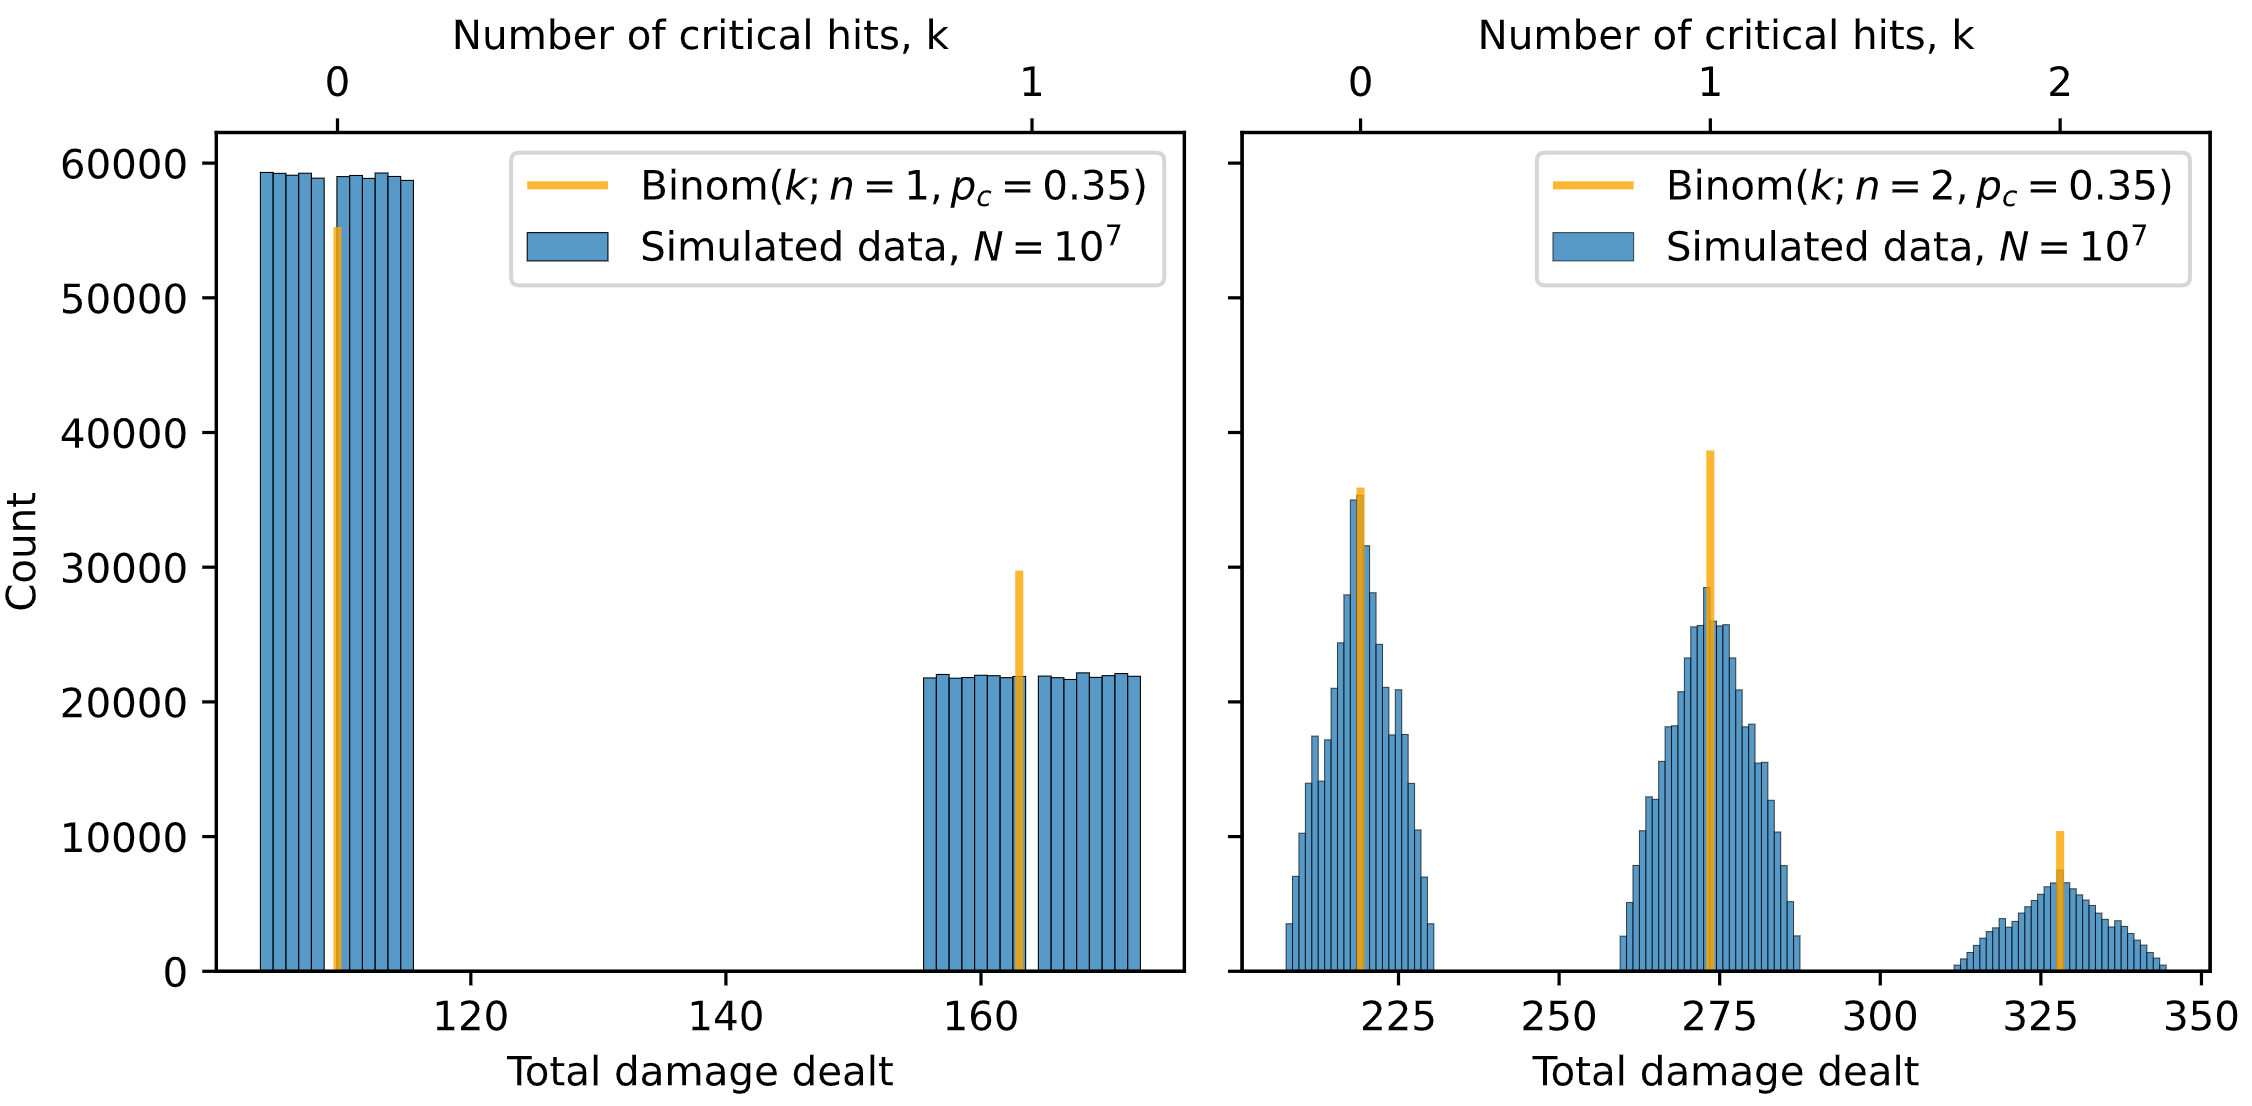
\includegraphics[width=0.95\linewidth]{img/binom-dmg-dist.PNG}
            \caption{Simulated damage distribution where $D_2 = 100$, $\lambda_c = 1500$, $p_c = 0.35$, and $\textbf{B} = [1.1]$. Figure 1a (left) shows the case where $n=1$ and Figure 1b (right) shows the case where $n=2$. Note the critical hit rate, $p_c$, and damage modifier, $\lambda_C$, are chosen arbitrarily.}\label{fig:CH-dmg-dist}
        \end{figure}

        Looking at Figure \ref{fig:CH-dmg-dist}a, the damage distribution for a normal hit can be thought of  rolling a (somewhat peculiar)  11-sided die with integer values ranging from 104--115, excluding 109. The damage distribution for landing a critical hit is like rolling a 16-sided die with integer values ranging from 156--172, excluding 164. The overall damage distribution is a mixture distribution, a linear combination of these sub-distributions,
        \begin{equation}
            P(x) = \sum_{k=1}^n w_k P_k(x)
        \end{equation}
        with the constraint that that $\sum_k w_k = 1$. Here, $n$ is the number of hits, $P_k$ is a discrete uniform with some missing integer values in its support, and the weights come from the binomial distribution, 

        \begin{equation}
            w_k = w_B(k;n, p) = \binom{n}{k}p_C^k (1-p_C)^{n-k}.
        \end{equation}
        
        % First, we define the range of the discrete uniform distribution for a normal hit, $a_N$ and $b_N$
        
        % \begin{equation}\label{eqn:normal-supp}
        %     \begin{split}
        %         a_N &= \lfloor 0.95 \lfloor D_2 \prod_{i}^{n_B}B_i \rfloor \rfloor \\
        %         b_N &= \lfloor 1.05 \lfloor D_2 \prod_{i}^{n_B}B_i \rfloor \rfloor
        %     \end{split}
        % \end{equation}

        % and the range of the discrete uniform distribution for a critical hit, $a_C$ and $b_C$

        % \begin{equation}\label{eqn:crit-supp}
        %     \begin{split}
        %         a_C &= \lfloor 0.95 \lfloor \lfloor \lfloor D_2 \lambda_C \rfloor / 1000 \rfloor \prod_{i}^{n_B}B_i \rfloor \rfloor \\
        %         b_C &= \lfloor 1.05 \lfloor \lfloor \lfloor D_2 \lambda_C \rfloor / 1000 \rfloor \prod_{i}^{n_B}B_i \rfloor \rfloor
        %     \end{split}
        % \end{equation}
        We can start to generalize from here. The damage sub-distribution for one normal hit is like rolling an $s_N$-sided die with some set of values that are not necessarily all integers in an interval. Similarly, the damage sub-distribution for one critical-hit is the same as rolling a $s_C$-sided die with some other set of values. The overall damage distribution is a sum of these sub-distributions with binomial weights. Figure \ref{fig:CH-dmg-dist}b with $n=2$ hits starts to get more interesting. For two normal hits, the sub-distribution is the sum of two $s_N$-sided dice rolls and the sub-distribution for two critical hits is the sum of two $s_C$-sided dice. For one critical hit and one normal hit, the sub-distribution is the sum of one $s_N$-sided die and one $s_C$-sided die, each with their respective value sets. For a skill that lands $n$ total hits, the damage sub-distribution of $k$ critical hits out of $n$ total hits will be the sum of $k$-fold $s_C$-sided dice rolls and $(n-k)$-fold $s_N$-sided dice rolls. 
        
        Although there is not a general formula for $s_i$, its value can readily be computed given $D_2$, $\lambda_C$, $p_C$, and \textbf{B}. The support for a single hit of type $i$ can be found by taking the set of unique integers in the sequence
        \begin{equation}\label{eqn:supp}
            D_i = \{\lfloor d  \prod_j B_j \rfloor \}
            % _{d = \lfloor 0.95 D_{3,i} \rfloor}^{\lfloor 1.05 D_{3,i} \rfloor} 
            \:\: d \in \{\lfloor 0.95 D_{3,i} \rfloor, \lfloor 1.05 D_{3,i} \rfloor \},   
        \end{equation}
        where $D_{3,i}$ is the damage after applying the appropriate damage modifiers for hit-type $i$. The value of $s_i$ is the cardinality (number of elements) of $D_i$, $|D_i|$. This dice-sum approach also works for damage dealt from DoT attacks. The major difference is that more gaps are introduced into the support of the damage because the uniform damage roll is applied before the hit type is determined, Figure \ref{fig:CH-dot-dmg-dist}.

        \begin{figure}[H]
            \centering
            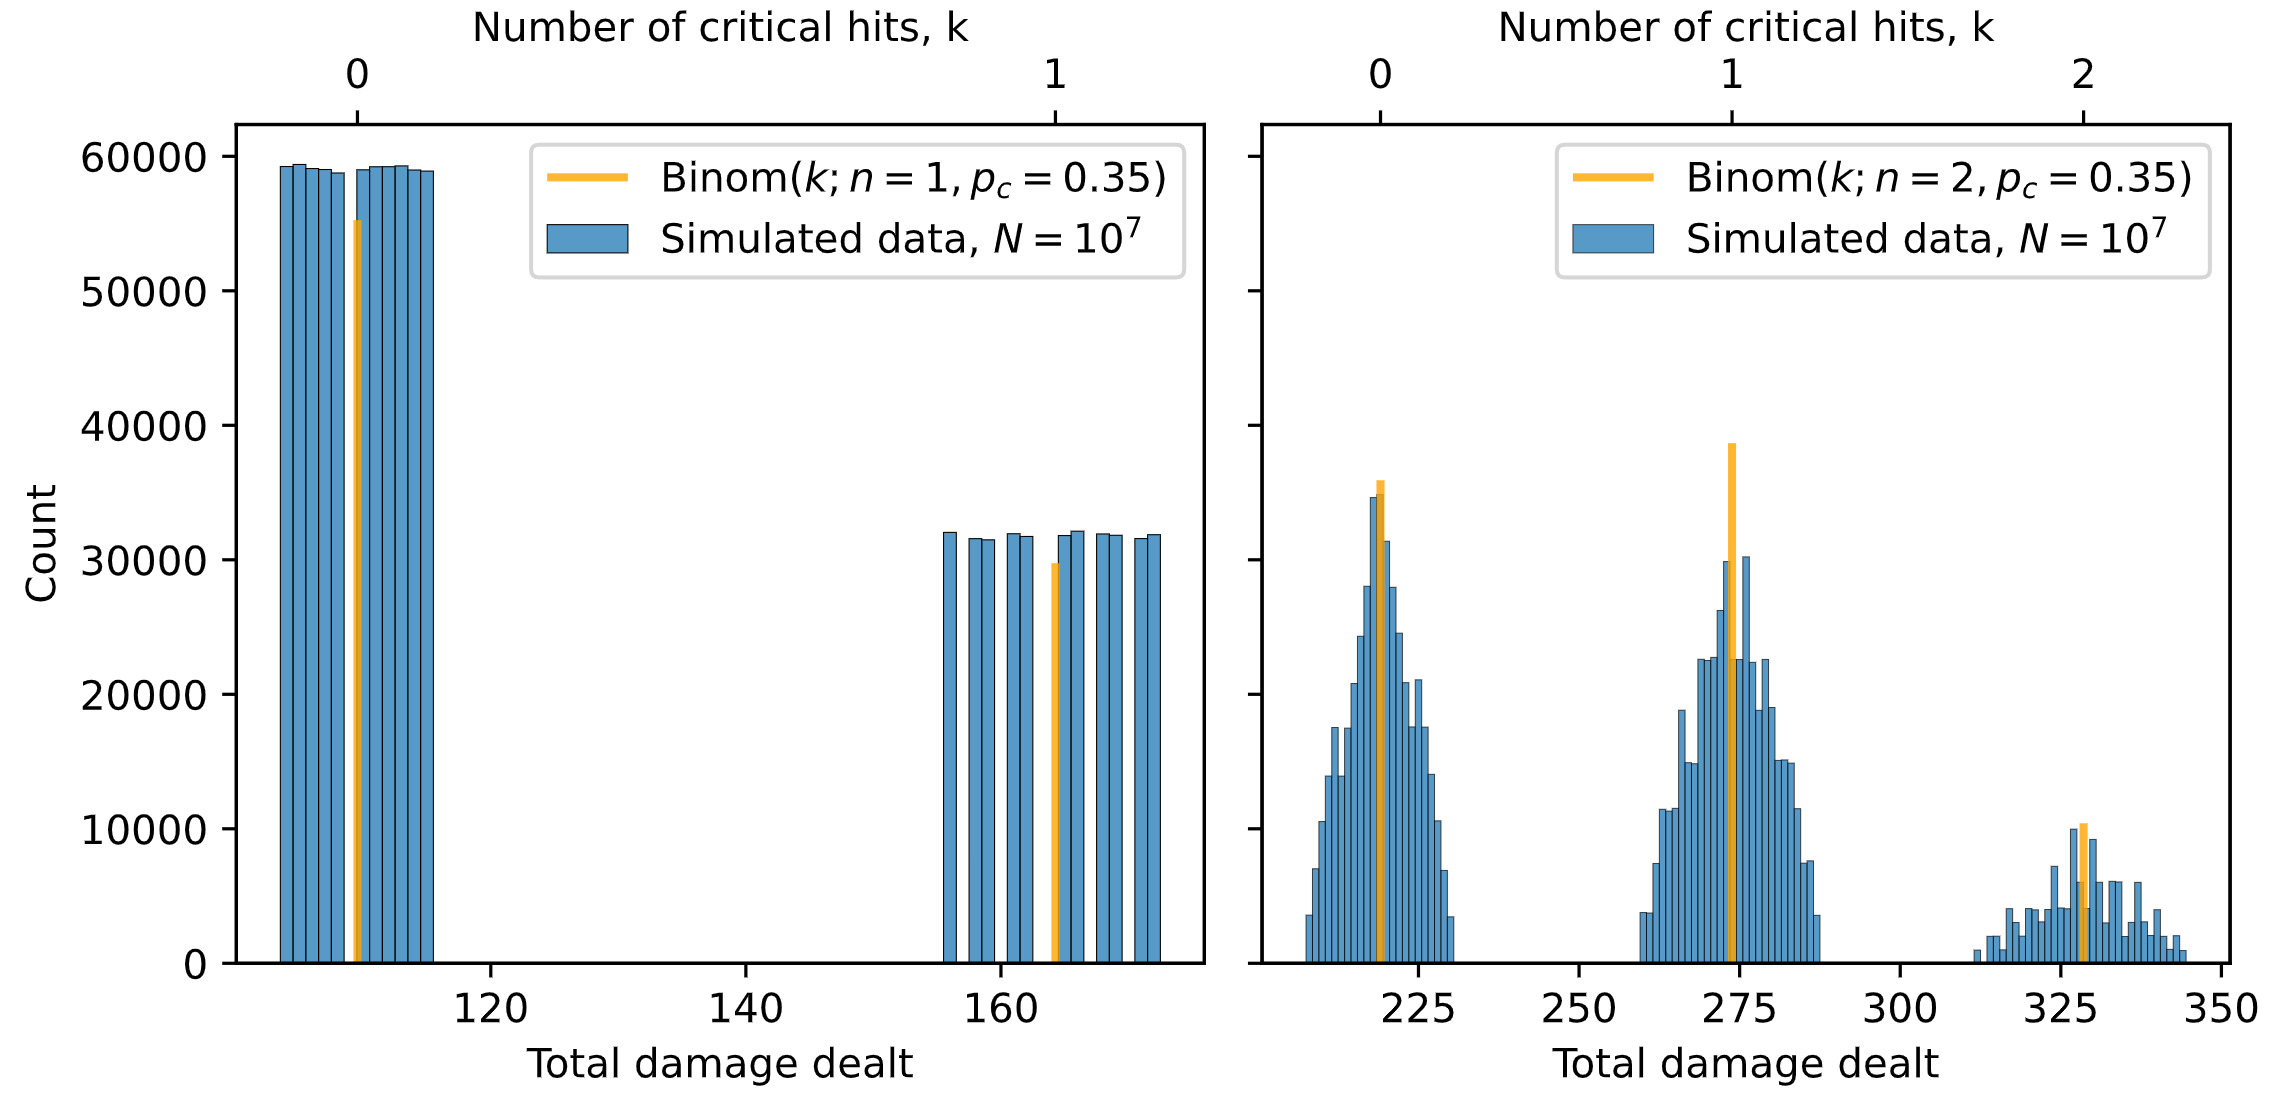
\includegraphics[width=0.95\linewidth]{img/binom-dot-dmg-dist.PNG}
            \caption{Simulated damage distribution from a DoT attack where $D_2 = 100$, $\lambda_c = 1500$, $p_c = 0.35$, and $\textbf{B} = [1.1]$. Figure \ref{fig:CH-dot-dmg-dist}a (left) shows the case where $n=1$ and Figure \ref{fig:CH-dot-dmg-dist}b (right) shows the case where $n=2$. Note the critical hit rate, $p_c$, and damage modifier, $\lambda_C$ are chosen arbitrarily.}\label{fig:CH-dot-dmg-dist}
        \end{figure}
        
        Because more gaps are introduced into the support, DoT attacks will have different $s_i$ values compared to non-DoT attacks. For a DoT attack landing hit type $i$, the support is the set of all unique integers in the sequence

        \begin{equation}\label{eqn:dot-supp}
            D_{DoT, i} = \{ \lfloor \lfloor \lfloor \lfloor \lfloor d \lambda_C \rfloor / 1000 \rfloor \lambda_D \rfloor / 100 \rfloor \prod_{j} B_j \rfloor \}
            % _{d = \lfloor 0.95 D_{2} \rfloor}^{\lfloor 1.05 D_{2} \rfloor} 
            \:\:\: d \in \{\lfloor 0.95 D_{2}\rfloor, \lfloor 1.05 D_{2} \rfloor\}
        \end{equation}
        where the appropriate damage modifiers for hit type $i$ applied. 
        % \begin{equation}\label{eqn:dot-supp}
        %     \begin{split}
        %         D_{i, DoT} = \{ &\lfloor \lfloor \lfloor \lfloor 0.95 D_{3, DoT} \lambda_C \rfloor / 1000 \rfloor \lambda_D \rfloor / 100 \rfloor \prod_{j}^{n_B}B_j \rfloor, \dots , \\
        %         &\lfloor \lfloor \lfloor \lfloor 1.05 D_{3, DoT} \lambda_C \rfloor / 1000 \rfloor \lambda_D \rfloor / 100 \rfloor \prod_{j}^{n_B}B_j \rfloor\}, 
        %     \end{split}           
        % \end{equation}

        The case with normal, critical, direct, and critical direct hits involves a sum of four different dice rolls, corresponding to each hit type. The weights in the mixture distribution will also be from the multinomial distribution, a generalization of the binomial distribution for any number of categories. The probability distribution of dice sums has been well-studied, but the general formula is cumbersome to work with because it includes many piecewise terms.\footnote{\url{https://mathworld.wolfram.com/Dice.html}} Most investigations also do not account for missing values in the range of point values. Since we are primarily interested in computing the mean and variance of the overall damage distribution, moment generating functions (MGFs) can be used instead, and will be much easier to define. The MGF for a each skill/ability can be individually defined and then combined to get an overall MGF for a rotation.

        \subsection{The mean and variance of a skill}

        Here, MGFs are briefly reviewed. The MGF for a discrete, random variable $X$ is

        \begin{equation}
            M_X(t) = \sum_{i \in \textrm{supp}(X)} p_i \exp[ti]
        \end{equation}
        where $i$ sums over the support of $X$ and $p_i$ is the probability for value $i$. Moments can be computed via the MGF by
        \begin{equation}\label{eqn:expected-deriv}
            E[X^n] = \left.\frac{d M_X(t)^n}{dt^n} \right|_{t=0},
        \end{equation}
        where $E$ is the expected value. Thus, the mean, variance, and skewness ($\gamma$) in terms of MGFs are

        \begin{equation}\label{eqn:mean-var}
            \begin{split}
                \mu &= E[X] = M^\prime_X(t=0) \\
                \sigma^2 &= E[X^2] - E[X]^2 = \left. M^{\prime\prime}_X(t) - M^\prime_X(t)^2 \right|_{t=0}\\
                \gamma &= \frac{E[X^3] - 3\mu\sigma^2 - \mu^3}{\sigma^3} = \frac{M^{\prime\prime\prime}(t=0) - 3\mu\sigma^2 - \mu^3}{\sigma^3}
            \end{split}
        \end{equation}
        The skewness measures how asymmetric the a distribution is. Negative skew typically occurs when the left tail of the distribution is longer and most of the mass is concentrated towards higher values. Positive skew typically occurs when the right tail of the distribution is longer and most of the mass is concentrated towards lower values.\footnote{See \url{https://en.wikipedia.org/wiki/Skewness} for a more detailed description on skewness.}
                
        We now define the MGF for our problem. Consider a single action landing $n$ total hits. A given damage sub-distribution will have $k$ critical hits and $n-k$ hits. Using the idea of sums of dice rolls, the corresponding MGF is
        % \begin{equation}\label{eqn:binom-sub-mgf}
        %     \frac{1}{s_C^k s_N^{n-k}} \left(\sum_{m=a_C}^{b_C} e^{m t}\right)^k \left(\sum_{m=a_N}^{b_N} e^{m t}\right)^{n-k}
        % \end{equation}

        % where $s_C^k = (b_C - a_C + 1)$ and $s_N^{n-k} = (b_N - a_N +1)^{n-k}$, the number of sides for each die. Because the distribution is uniform, all values of a given hit type have the same probability of $1/s_i$. The exponents $k$ and $n-k$ represent summing $k$-fold $s_C$-sided dice rolls and $n-k$-fold $s_N$-sided dice rolls, respectively. A more detailed explanation of constructing the MGF for these sorts of distributions can can be found in Signh et al. 
        
        % Eqn. \ref{eqn:binom-sub-mgf} is the MGF for one sub-distribution of a particular number of critical hits. The MGF of the mixture distribution of a skill, $M_S(t)$, enumerates over all hit-type combinations and can be expressed by summing with binomial weights.

        % \begin{equation}\label{eqn:binom-skill-mgf}
        %     M_S(t) = \sum_{k=0}^{n} \frac{w_B(k;n,p_C)}{s_C^k s_N^{n-k}} \left(\sum_{m=a_C}^{b_C} e^{m t}\right)^k \left(\sum_{m=a_N}^{b_N} e^{m t}\right)^{n-k}
        % \end{equation}

        % The mean and variance can be computed from eqn. \ref{eqn:mean-var}. Evaluating the first derivative at $t=0$ to get the mean and simplifying is

        % \begin{equation}
        %     \mu_S = \frac{1}{2} \sum_{k=0}^n w_B(k;n,p_C) (k(a_C + b_C) + (n-k)(a_N + b_N))
        % \end{equation}

        % The variance is

        % \begin{equation}
        %     \begin{split}
        %         \sigma_S^2 &= \frac{1}{12} \sum_{k=0}^n [w_B(k;n,p_C) (k (a_C + a_N - b_C - b_N - 2) \\ 
        %         &\qquad\qquad\qquad\times (a_C + b_N - b_C - b_N) +n(a_N - b_n - 2)(a_N - b_N))] - \mu_S^2
        %     \end{split}      
        % \end{equation}

        
        % The MGF for damage due to a DoT attack ticking $n$ times with $k$ critical ticks and $n-k$ normal ticks is

        \begin{equation}\label{eqn:binom-sub-mgf}
            \frac{1}{s_C^k s_N^{n-k}} \left( \sum_{m \in D_{C}} e^{m t} \right)^n 
            \left( \sum_{m \in D_{N}} e^{m t} \right)^{n-k}.
        \end{equation}
        Here, the sums enumerate over the support for a single hit of a given type, $D_i$. Because the distribution is uniform, all values of a given hit type have the same probability of $1/s_i$. The exponents $k$ and $n-k$ represent summing $k$-fold $s_C$-sided dice rolls and $(n-k)$-fold $s_N$-sided dice rolls, respectively. A more detailed explanation of constructing the MGF for sums of dice can can be found in Signh et al.\footnote{Singh, A. K., Dalpatadu, R. J., \& Lucas, A. F. (2011). The Probability Distribution of the Sum of Several Dice: Slot Applications. UNLV Gaming Research \& Review Journal. \url{https://digitalscholarship.unlv.edu/grrj/vol15/iss2/10/}} Eqn. \ref{eqn:binom-sub-mgf} applies for both DoT and non-DoT attacks, but the appropriate value of $s_i$ must be used. The MGF for the distribution of damage dealt is then
        \begin{equation}\label{eqn:binom-mgf}
            \sum_{k=0}^{n}
            \frac{w_B(k;n,p_C)}{s_C^k s_N^{n-k}} \left( \sum_{m \in D_{C}} e^{m t} \right)^n 
            \left( \sum_{m \in D_{N}} e^{m t} \right)^{n-k}
        \end{equation}
        The mean and variance can be computed from eqn. \ref{eqn:mean-var}. Evaluating the first derivative at $t=0$ to get the mean and simplifying yields
        \begin{equation}\label{eqn:binom-mean}
            \mu_{S} = \sum_{k=0}^n w_B(k;n,p_C) \left[k \frac{Z_C}{s_C} + (n-k) \frac{Z_N}{s_N}\right]
        \end{equation}
        Where $Z_i$ is the sum of all values in the support for hit-type $i$, $Z_i = \sum_{m \in D_{i}} m $. The variance is
        \begin{equation}\label{eqn:binom-var}
            \begin{split}
                \sigma_{S}^2 = \sum_{k=0}^n w_B(k)   & \left[ \frac{n^2 Z_N^2}{s_N^2} \right.+ k^2 \left(\frac{Z_C^2}{s_C^2} - \frac{2 Z_C Z_N}{s_C s_N} + \frac{Z_N^2}{s_N^2}\right)  \\
                & \: + k \left(-\frac{Z_C^2}{s_C^2} + \frac{Z_{C,2}}{s_C} + \frac{Z_N^2}{s_N^2} + 
                n \left(\frac{2 Z_C Z_N}{s_C s_N} - \frac{2 Z_N^2}{s_N^2}\right) - \frac{Z_{N,2}}{s_N}\right) \\
                & \: \left.+ n \left(\frac{Z_{N,2}}{s_N} - \frac{Z_N^2}{s_N^2} \right)\right] - \mu_{S}^2              
            \end{split}
        \end{equation}
        where $Z_{i,2} = \sum_{m \in D_{i}} m^2$. The skewness is computed in a similar way, but the formula will not be typeset because it is significantly longer and the exact form is not illustrative. An image of the formula for $M^{\prime\prime\prime}_S(t)$ can be found at the end, Figure \ref{fig:binom-3rd-deriv}.
        % Eqns. \ref{eqn:binom-mean} and \ref{eqn:binom-var} give the mean and variance for a single skill/ability landing $n$ hits.

        \subsection{The mean and variance of a rotation}\
        Until now, we have only dealt with computing the mean and variance of a single attack landing $n$ total hits. Ultimately, we want to compute the mean and variance of a rotation, a collection of skills each landing their respective number of total hits. Although skills in a rotation are performed in a specific order, the damage they deal are independent from each other.\footnote{This is still true for combos, where additional damage is granted for successfully completing attacks in a specific order. The additional damage granted is a conditional probability distribution, given the prior hit in the combo was successfully performed.} The moment generating function for a sum of independent variables is
        
        \begin{equation}
            M_R(t) = \prod_{m=0}^{n_s} M_{S_m}(t),
        \end{equation}
        where $M_R(t)$ is the MGF for a rotation, $n_s$ is the number of skills in a rotation, and $M_{S_m}(t)$ is the MGF for skill $m$. For independent variables, it can be shown that the mean, variance, and skewness for $M_R(t)$ is
        
        \begin{equation}\label{eqn:sum-of-stuff}
            \begin{split}
                \mu_R &= \sum_{m=0}^{n_s} \mu_m \\
                \sigma^2_R &= \sum_{m=0}^{n_s} \sigma_{m}^2 \\
                \gamma_R &= \frac{\sum_m M_m^{\prime\prime\prime}(t=0) - 3\mu_m \sigma_m^2 - \mu_m^3}
                {\left(\sum_m \sigma_{m}^2\right)^{3/2}} 
            \end{split}
        \end{equation}
        where $n_s$ is the total number of unique attacks performed and $\mu_m$ and $\sigma_m^2$ are the mean and variance for skill $m$, respectively. The mean and variance follow the well-known sum of mean and sum of variance formulae for independent variables. The rotation skewness is not exactly a sum of the constituent skewnesses because of the denominator.


    \section{Accounting for normal, critical, direct, and critical-direct hits}
        Adding the possibility direct hits and critical-direct hits does not change the approach to characterizing the damage distribution. However, instead of summing two dice to account for the uniform damage rolls, four dice are summed. The number of each hit types is $\textbf{x} = [x_N, x_C, x_D, x_{CD}]$,\footnote{The order of hit types for vectors will always be normal, critical, direct, and critical-direct.} where $\sum_i x_i = n$. The probability for each hit type is $\textbf{p} = [1 - p_C - p_D + p_{CD}, p_C - p_C p_D, p_D  - p_C p_D, p_C p_D]$. For critical and direct hits, subtracting $p_C p_D$ prevents over-counting critical or direct hits that became critical-direct hits. We can visualize the damage distribution for a single skill landing $n=1$ hits and $n=2$ hits.

        \begin{figure}[H]
            \centering
            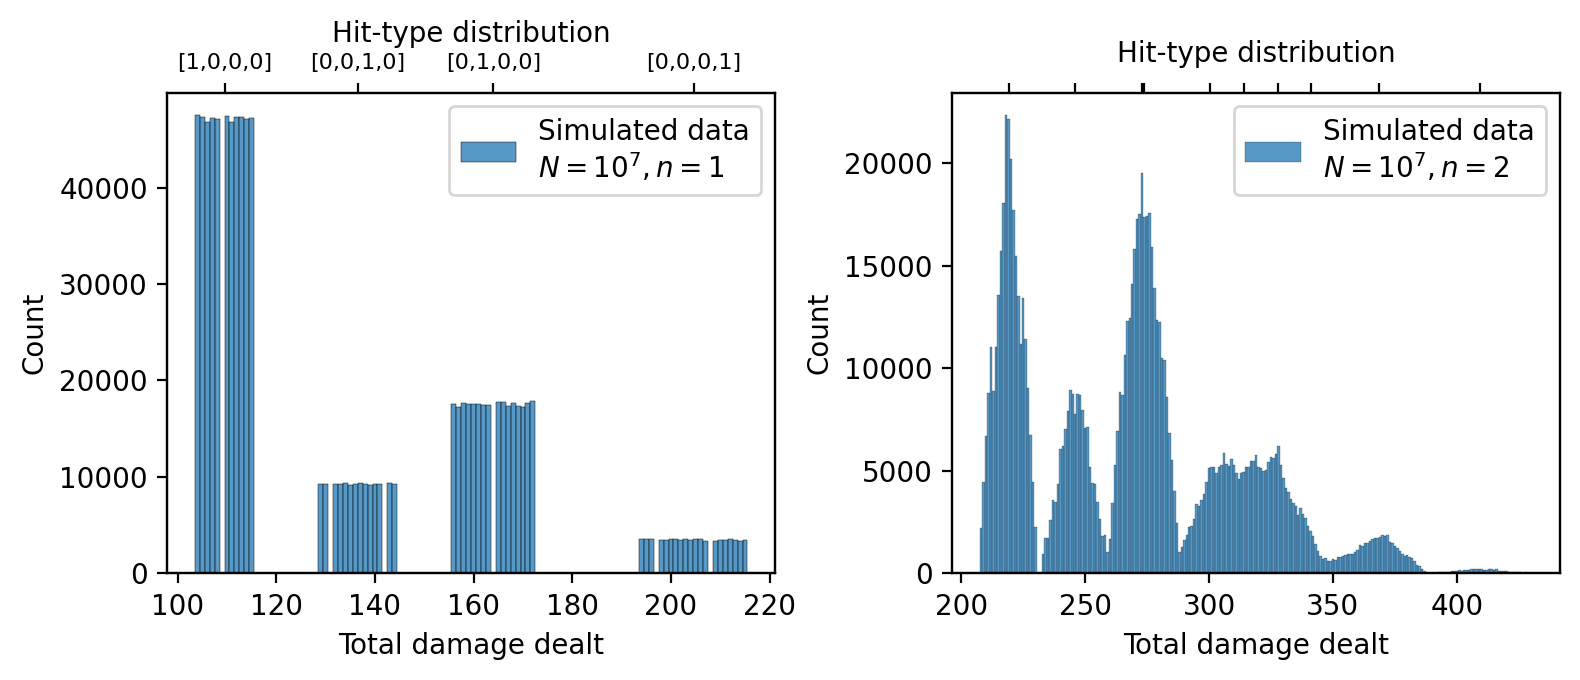
\includegraphics[width=0.90\linewidth]{img/multi-dmg-dist.PNG}
            \caption{Simulated damage distribution where $D_2 = 100$, $\lambda_c = 1500$, $\lambda_D = 125$, $\textbf{p} = [0.38, 0.35, 0.2 , 0.07]$, and $\textbf{B} = [1.1]$. Figure 1a (left) shows the case where $n=1$ and the upper x-axis shows the hit-type distribution. Figure 1b (right) shows the case where $n=2$. Note the critical hit rate, $p_c$, direct hit rate, $p_D$, and damage modifier, $\lambda_C$ are chosen arbitrarily.}\label{fig:multi-dmg-dist}
        \end{figure}

        Even with just two hits, the sub-distributions already start to overlap each other. The damage distribution for DoT attacks is similar, but with more missing values in the support,

        \begin{figure}[H]
            \centering
            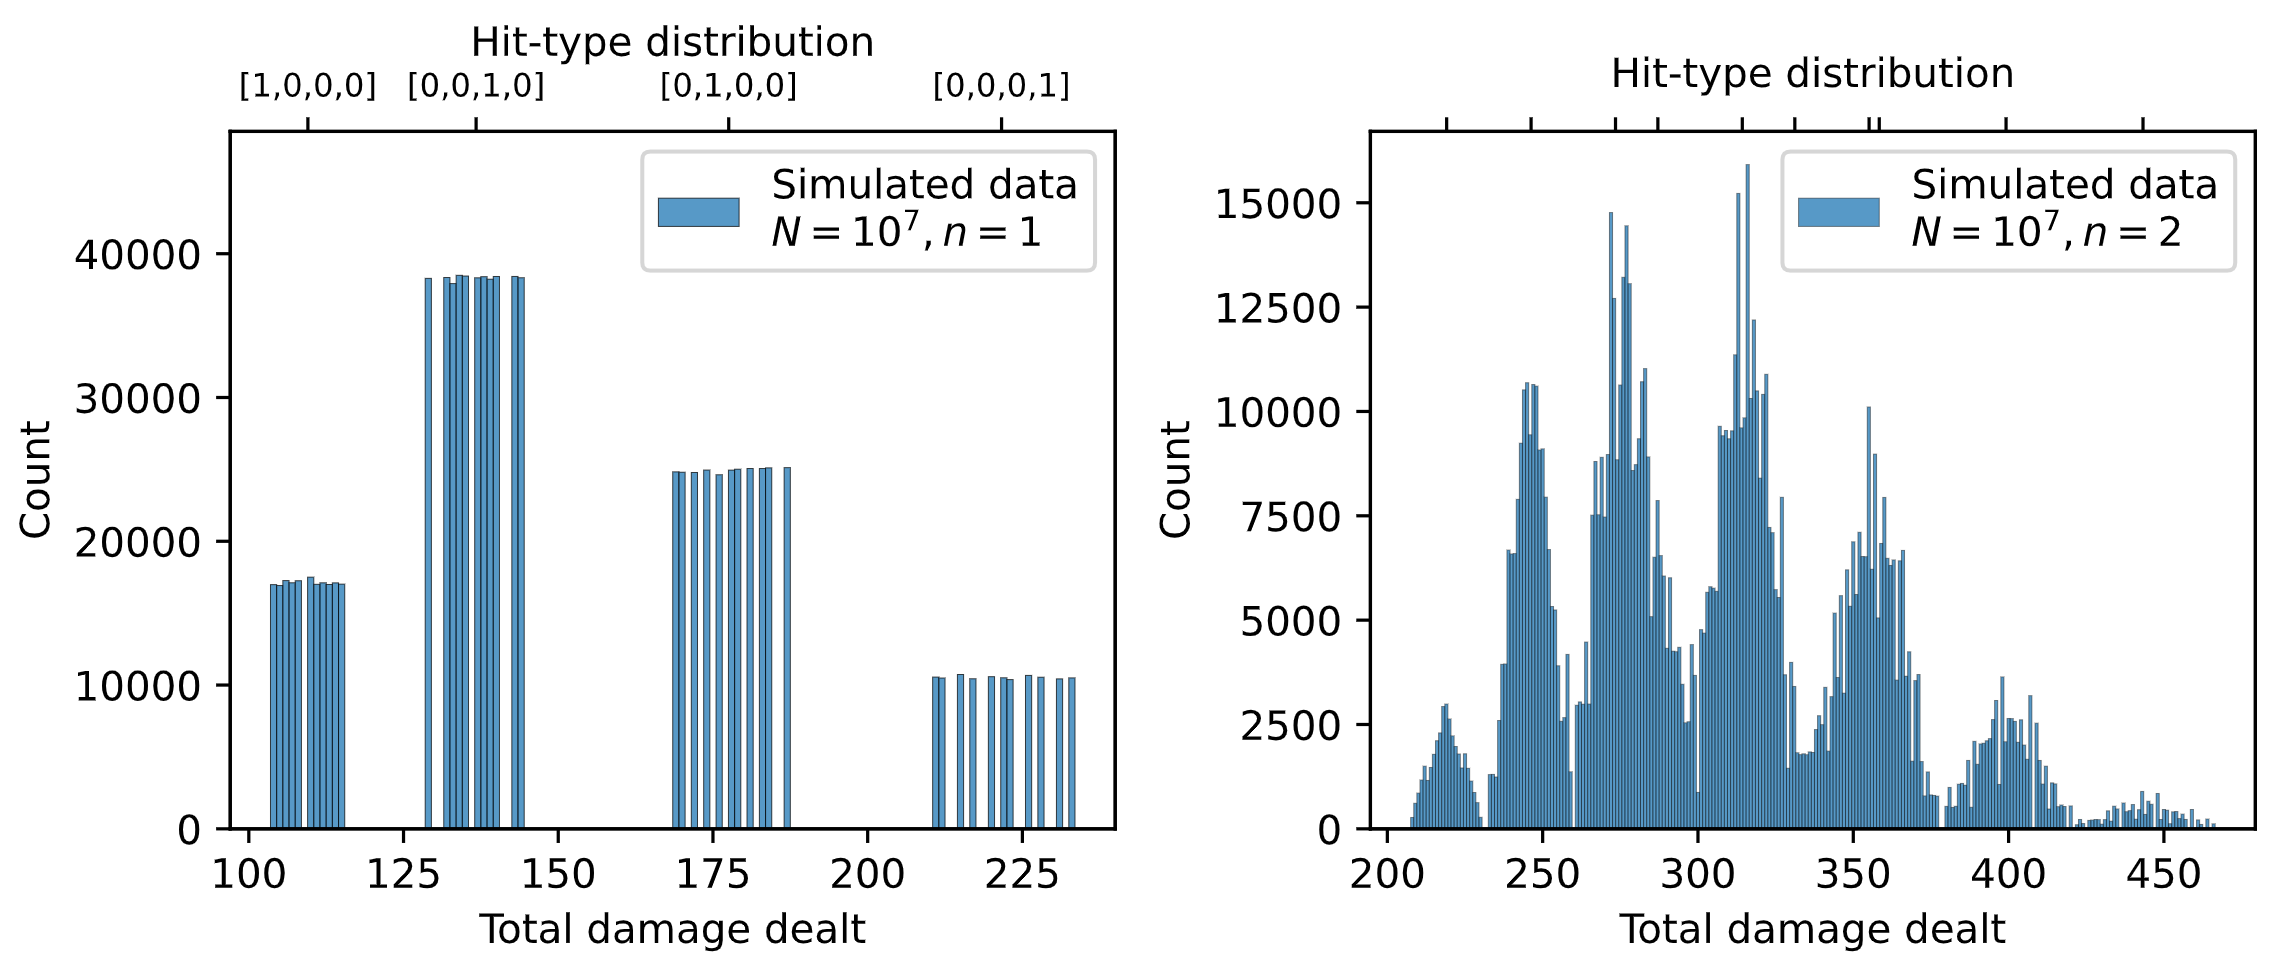
\includegraphics[width=0.90\linewidth]{img/multi-dot-dmg-dist.PNG}
            \caption{Simulated DoT distribution where $D_2 = 100$, $\lambda_c = 1500$, $\lambda_D = 125$, $\textbf{p} = [0.38, 0.35, 0.2 , 0.07]$, and $\textbf{B} = [1.1]$. Figure 1a (left) shows the case where $n=1$ and the upper x-axis shows the hit-type distribution. Figure 1b (right) shows the case where $n=2$. Note the critical hit rate, $p_c$, direct hit rate, $p_D$, and damage modifier, $\lambda_C$ are chosen arbitrarily.}\label{fig:multi-dot-dmg-dist}
        \end{figure}
        
        The supports of direct hit and critical-direct hit distributions are computed in the same manner as eqns. \ref{eqn:supp} and \ref{eqn:dot-supp}. The MGF allowing for direct hits and critical-direct hits is similar to eqn. \ref{eqn:binom-mgf}, with two additional dice roll sums added to account for the two new hit types,
        % \begin{equation}\label{eqn:direct-supp}
        %     \begin{split}
        %         a_C &= \lfloor 0.95 \lfloor \lfloor \lfloor D_2 \lambda_D \rfloor / 100 \rfloor \prod_{i}^{n_B}B_i \rfloor \rfloor \\
        %         b_C &= \lfloor 1.05 \lfloor \lfloor \lfloor D_2 \lambda_D \rfloor / 100 \rfloor \prod_{i}^{n_B}B_i \rfloor \rfloor                
        %     \end{split}
        % \end{equation}
        % and
        % \begin{equation}\label{eqn:cd-supp}
        %     \begin{split}
        %         a_{CD} &= \lfloor 0.95 \lfloor \lfloor \lfloor \lfloor D_2 \lambda_C \rfloor / 1000 \rfloor 100 \rfloor \prod_{i}^{n_B}B_i \rfloor \rfloor \\
        %         b_{CD} &= \lfloor 1.05 \lfloor \lfloor \lfloor \lfloor D_2 \lambda_C \rfloor / 1000 \rfloor 100 \rfloor \prod_{i}^{n_B}B_i \rfloor \rfloor                
        %     \end{split}
        % \end{equation}

        % The MGF for $n$ non-DoT hits is

        % \begin{equation}\label{eqn:multi-mgf}
        %     M_S(t) = \mathop{\sum_{i=0}^n \sum_{i=j}^n \sum_{k=0}^{n} \sum_{l=0}^n}_{i+j+k+l \le n} 
        %     \frac{w_M(\textbf{x}, \textbf{p}; n)}{s_N^{i} s_C^j s_D^{k} s_{CD}^{l}} 
        %     \left(\sum_{m=a_N}^{b_N} e^{m t}\right)^i 
        %     \left(\sum_{m=a_C}^{b_C} e^{m t}\right)^{j} 
        %     \left(\sum_{m=a_D}^{b_D} e^{m t}\right)^k
        %     \left(\sum_{m=a_CD}^{b_{CD}} e^{m t}\right)^l
        % \end{equation}
        % where $s_i = (b_i - a_i + 1)$. 
        \begin{equation}\label{eqn:multi-dot-mgf}
            M_S(t) = \mathop{\sum_{i=0}^n \sum_{i=j}^n \sum_{k=0}^{n} \sum_{l=0}^n}_{i+j+k+l \le n} 
            \frac{w_M(\textbf{x}, \textbf{p}; n)}{s_N^{i} s_C^j s_D^{k} s_{CD}^{l}} 
            \left(\sum_{m \in D_N} e^{m t}\right)^i 
            \left(\sum_{m \in D_C} e^{m t}\right)^{j} 
            \left(\sum_{m \in D_D} e^{m t}\right)^k
            \left(\sum_{m \in D_{CD}} e^{m t}\right)^l
        \end{equation}
        The four sums iterate over all hit-type combinations (\textit{i.e.}, $\textbf{x} = [i, j, k, l]$) and the restriction on the sums ensures that the sum of indices do not exceed $n$. The weights $w_M$ are from the multinomial distribution, a generalization of the binomial distribution for more than two outcomes,
        \begin{equation}
            w_M(\textbf{x}, \textbf{p};n) =  \frac{n!}{\prod_{i=1}^{4} x_i!}\prod_{i=1}^{4} p_i^{x_i}
        \end{equation}
        % Note that there is no general formula for $s_m$ or the support of $s_m$ for eqn. \ref{eqn:multi-dot-mgf}, so these must be computed given values of $D_2$, $\lambda_C$, and $\lambda_D$. For non-DoT hits, the mean is
        % \begin{equation}\label{eqn:multi-skill-mean}
        %     \mu_S = 
        %     \frac{1}{2} \multisum w_M(\textbf{x}, \textbf{p};n) \left[
        %     i(a_N + b_N) +  j(a_C + b_C) +  k(a_D + b_D) + 
        %     l(a_{CD} + b_{CD}) \right]
        % \end{equation}
        % The variance is
        % \begin{equation}
        %     \begin{split}
        %         \sigma_S^2 = \multisum &w_M(\textbf{x}, \textbf{p};n) \left[\frac{1}{4} (a_N + b_N)^2 i^2  \right.\\
        %         & + \frac{1}{4} (a_C + b_C)^2 j^2 + \frac{1}{4} (a_D + b_D)^2 k^2 \\
        %         & + \frac{1}{12} (-2 + a_{CD} - b_{CD}) (a_{CD} - b_{CD}) l + \frac{1}{4} (a_{CD} + b_{CD})^2 l^2 \\
        %         & + j \left(\frac{1}{12} (-2 + a_C - b_C) (a_C - b_C) \right. \\
        %         & \left. +\frac{1}{2} (a_C + b_C) (a_D + b_D) k + \frac{1}{2} (a_C + b_C) (a_{CD} + b_{CD}) l\right) \\
        %         & + k \left(\frac{1}{12} (-2 + a_D - b_D) (a_D - b_D) + \frac{1}{2} (a_{CD} + b_{CD}) (a_D + b_D) l\right) \\
        %         & + i \left(\frac{1}{12} (-2 + a_N - b_N) (a_N - b_N) + \frac{1}{2} (a_C + b_C) (a_N + b_N) j \right.\\
        %         & \left. \left. + \frac{1}{2} (a_D + b_D) (a_N + b_N) k + \frac{1}{2} (a_{CD} + b_{CD}) (a_N + b_N) l\right)\right] - \mu_S^2.
        %     \end{split}
        % \end{equation}
        Using eqn. \ref{eqn:mean-var}, the mean when $n$ hits are landed is
        \begin{equation}
            \mu_S = \multisum w_M(\textbf{x}, \textbf{p};n)\left[i \frac{Z_N}{s_N} + j\frac{Z_C}{s_C} + k \frac{Z_D}{s_D} + l \frac{Z_{CD}}{s_{CD}}\right].
        \end{equation}
        and the variance is
        \begin{equation}
            \begin{split}
                \sigma_S^2 = \multisum w_M(\textbf{x}, \textbf{p};n) & \left[ \frac{j^2 Z_C^2}{s_C^2} + \frac{l^2 Z_{CD}^2}{s_{CD}^2} + \frac{k^2 Z_D^2}{s_D^2} + \frac{i^2 Z_N^2}{s_N^2} \right. \\
                &+ i \left(\frac{2 j Z_C Z_N}{s_C s_N} + \frac{2 l Z_{CD} Z_N}{s_{CD} s_N} + \frac{2 k Z_D Z_N}{s_D s_N} - \frac{Z_N^2}{s_N^2} + \frac{Z_{N,2}}{s_N}\right) \\
                & +j \left(\frac{Z_{C,2}}{s_C} - \frac{Z_C^2}{s_C^2}  + \frac{2 l Z_C Z_{CD}}{s_C s_{CD}} + \frac{2 k Z_C Z_D}{s_C s_D}\right) \\
                & + k \left(\frac{2 l Z_{CD} Z_D}{s_{CD} s_D} - \frac{Z_D^2}{s_D^2} + \frac{Z_{D,2}}{s_D}\right)  \\ 
                & \left. + l \left(\frac{Z_{CD,2}}{s_{CD}} - \frac{Z_{CD}^2}{s_{CD}^2}\right)\right] - \mu_{S}^2
            \end{split}
        \end{equation}
        As before the formula for skewness will not be typeset because it is even longer. An image of the formula for $M^{\prime\prime\prime}_S(t)$ can be found at the end, Figure \ref{fig:multi-3rd-deriv}.

        Eqn. \ref{eqn:sum-of-stuff} still applies for combining the means and variance from a set of skills into the mean and variance of a rotation, respectively.

        \section{Results: Computing and comparing the mean and variance of rotations}

        Now that all the machinery for computing the mean and variance of damage distributions is developed, they can be tested on some simple ``rotations''. This section aims to only illustrate the framework using simple sequence of skills that are representative of some jobs and not an attempt to fully model all aspects of a specific job. The first rotation is a single attack skill and a DoT skill, similar to a healer. The second rotation is a ``1-2-3'' combo, a DoT, a persistent 10\% damage buff, and a periodic heavy-hitting attack. This rotation could be thought of as a tank rotation or a DPS rotation lacking off global cooldowns. For each rotation, three cases will be investigated: (i) hit types can be normal or critical, (ii) hit types can be normal, critical, direct, or critical-direct (CD), and (iii) hit types can be be normal, critical, or direct.\footnote{Comparing case (i) to cases (ii) and (iii) should not be thought of as comparing a build with low direct hit rate, because the direct hit rate is just deleted. In reality, the total number of stats is roughly constant and would those deleted stat points would likely be reallocated to another stat like determination or critical hit.} Results will also be converted from damage dealt into damage per second (DPS) by assuming a 2.50 second GCD. Values of $D_2$ will be chosen to be similar to $D_2$ values seen in patch 5.5. 
        
        \subsection{Rotation 1}
            Here, we look at a rotation containing a single attack and a DoT. For Rotation 1, the critical hit stat is 3731 and direct hit rate stat is 1280, which leads to $\lambda_C = 1603$, $\lambda_D = 125$, and $\textbf{p} = [0.635, 0.215, 0.112, 0.038]$. Removing the possibility of no direct-crit hits results in $\textbf{p} = [0.597, 0.253, 0.150, 0]$. Values of $D_2$ for each attack and the number of each attacks are listed in Table \ref{t:rot1}

            \begin{table}[H]
                \centering
                \caption{$D_2$ values and total number of hits action $i$ lands for Rotation 1.}\label{t:rot1}
                \begin{tabular}{@{}lll@{}}
                \toprule
                Action & $D_2(i)$ & $n(i)$ \\ \midrule
                1       & 20,000 & 50   \\
                2 (DoT) &  5,000 & 50   \\ \bottomrule
                \end{tabular}
            \end{table}

            If 50 are hits on the global cooldown, the total time elapsed is $t = 2.50 s \times 50 =125s$, and the DPS is $D / t$. Figure \ref{fig:rot-1} shows results for the three cases described above. 
            
            \begin{figure}[H]
                \begin{subfigure}[b]{0.49\textwidth}
                    \centering
                    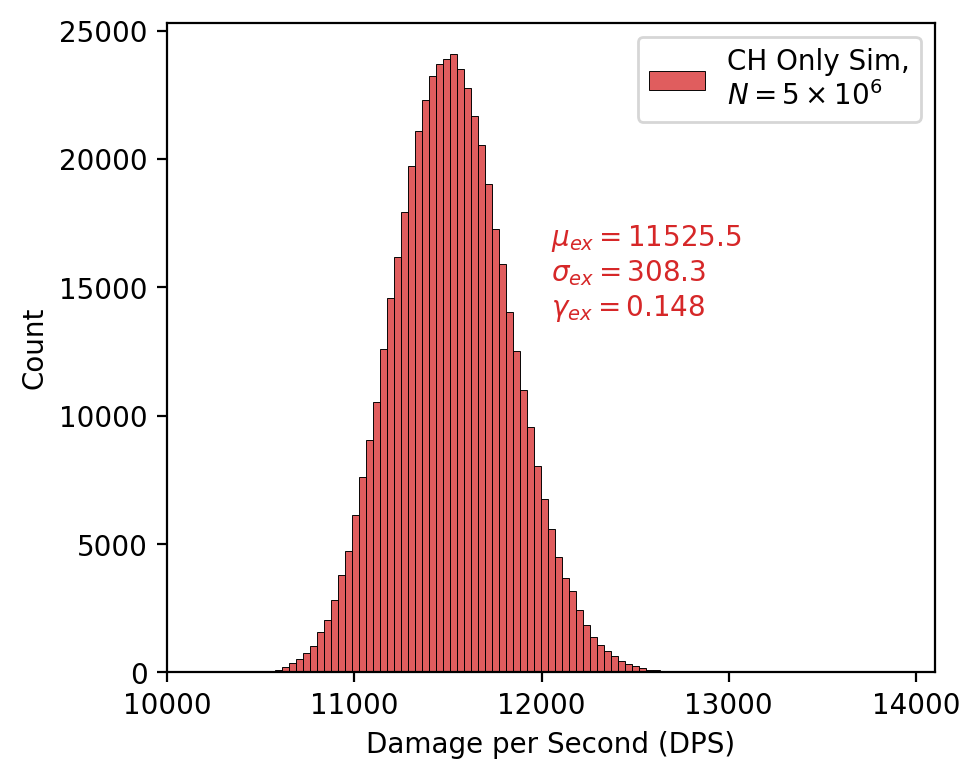
\includegraphics[width=\textwidth]{img/rotation-1-CH.PNG}
                \end{subfigure}
                \hfill
                \begin{subfigure}[b]{0.49\textwidth}
                    \centering
                    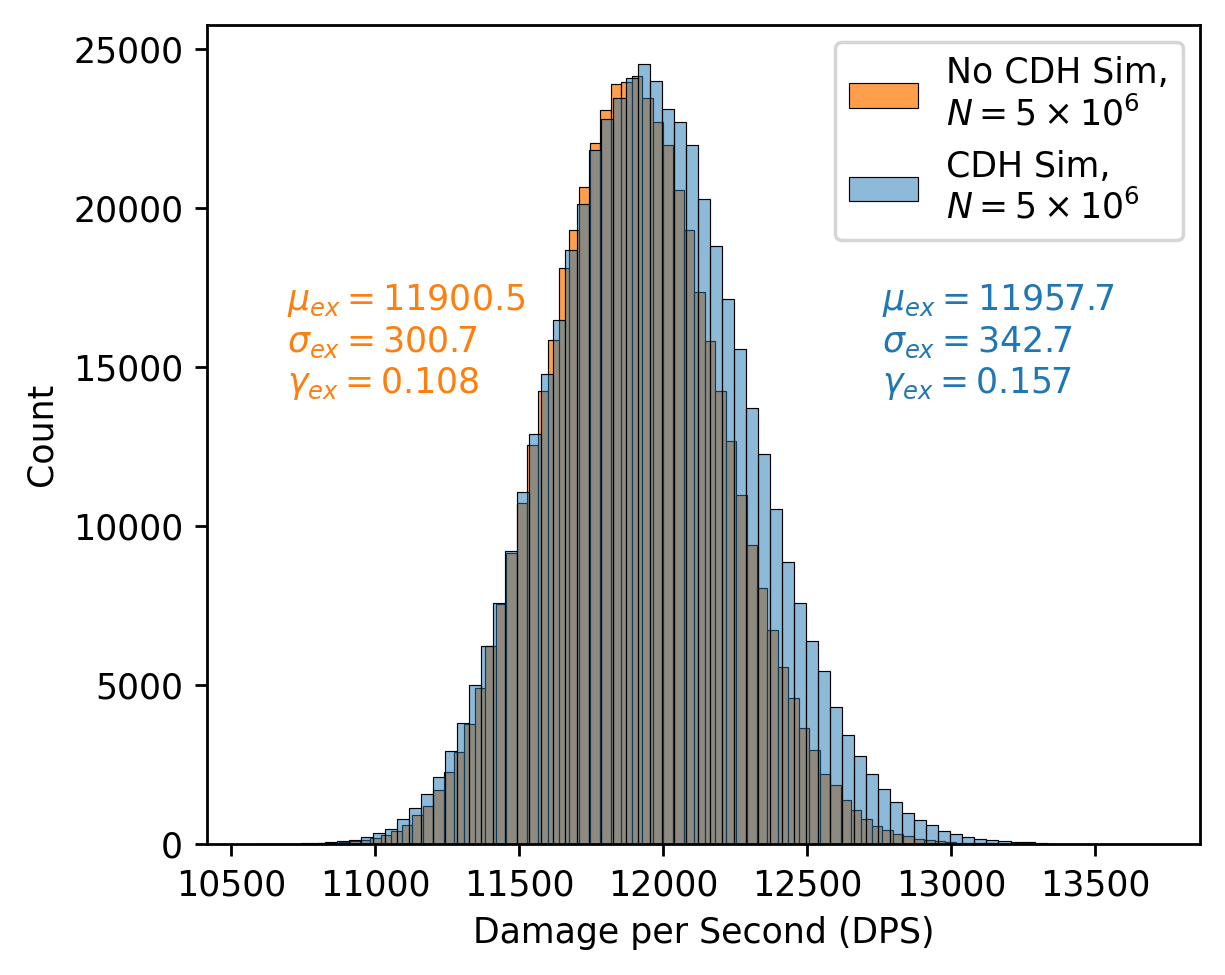
\includegraphics[width=\textwidth]{img/rotation-1.PNG}
                \end{subfigure}
                \caption{Simulated DPS distributions for different hit type combinations for Rotation 1. Each skill is simulated $5 \times 10^6$ times. The exact mean, standard deviation, and skewness for each combination are also shown.}\label{fig:rot-1}
            \end{figure}

            The simulations were performed to mainly illustrate the shape of the DPS distribution and to compare sample estimates of the mean and standard deviation against the exact solutions. The exact mean, standard deviation, and skewness are also within $1\%$ of the sample estimates, which is likely due to sampling error. For a large number of hits, both sums of uniform distributions and the binomial/multinomial distribution distribution tends towards a normal distribution. Although the multinomial distribution is four-dimensional here, the final result is one-dimensional because the hit-type distribution is projected onto DPS. Both sums and convolutions of normally distributed variables result in a normally distributed variable, so the histogram shapes in Figure \ref{fig:rot-1} are reasonable.  For a small number of hits, such as an opener or a specific phase in the rotation (or Figure \ref{fig:multi-dmg-dist}), the DPS distribution will not follow a normal distribution. To a lesser extent, this can also be seen in Figure \ref{fig:rot-1} when CD hits are included/excluded. The skewness increases from $0.11$ without critical direct hits to $0.16$ with CD hits. 

            For all three cases, the mean increases as the number of hit-type increases. This is expected because the other hit types deal more damage than normal hits, and their addition lowers the chance of a normal hit landing. Directly comparing standard deviations is not the most apt comparison because the addition of hit types affects both the mean and standard deviations. We are more generally interested in the how the addition of hit types affects the variability, the degree of how stretched a distribution is. The coefficient of variation, $c_v$ is a more convenient measure of variability here because it is a dimensionless quantity that accounts for changes in both the mean and the standard deviation. It can also be thought of as a relative standard deviation,

            \begin{equation}
                c_v = \frac{\sigma}{\mu}.
            \end{equation}
            A change that increases $c_v$ increases the standard deviation by a greater magnitude than the mean. Conversely, a change that decreases $c_v$ means the standard deviation was increased by a lesser amount than the mean was. Table \ref{t:r1-cv} shows the coefficient of variations for the three cases and the percent changes relative to the case with only normal or critical hits.

            \begin{table}[H]
                \centering
                \caption{Coefficient of variation and skewness for different hit-type combinations of Rotation 1. The percent change relative to only normal and critical hits are also shown.}\label{t:r1-cv}
                \begin{tabular}{@{}lllll@{}}
                    \toprule
                    Hit types present & $c_v$ & \% Change & $\gamma$ & \% Change \\ \midrule
                    NH, CH            & 0.027 & 0.0\%     & 0.148    & 0.0\%     \\
                    NH, CH, DH        & 0.025 & -5.2\%    & 0.108    & -27.3\%   \\
                    All               & 0.029 & 7.5\%     & 0.157    & 5.7\%     \\ \bottomrule
                    \end{tabular}
                \end{table}
            
            The addition of direct hits and critical direct hits increases the standard deviation of the DPS distribution by 5\% more than the mean increased. If CD hits are removed, $c_v$ decreases by 7.5\% relative to the NH/CH only case. For this set of stats and rotation, including CD hits increases variability of the DPS distribution by an appreciable margin. 

        \subsection{Rotation 2}
            Here, we look at a rotation containing ``1-2-3'' combo, a DoT, a persistent 10\% damage buff, and a periodic heavy-hitting attack. For rotation 2, the critical hit stat is 4069 and direct hit rate stat is 2919. This leads to $\lambda_C = 1623$, $\lambda_D = 125$, and $\textbf{p} = [0.412, 0.158, 0.308, 0.116]$. Removing the possibility of no direct-crit hits results in $\textbf{p} = [0.304, 0.273, 0.423, 0]$. Values of $D_2$ for each attack and the number of each attacks are listed in Table \ref{t:rot2}.

        \begin{table}[H]
            \centering
            \caption{$D_2$ values used and total number of hits action $i$ lands for rotation 2.}\label{t:rot2}
            \begin{tabular}{@{}lll@{}}
            \toprule
            \multicolumn{1}{l}{Action} & \multicolumn{1}{l}{$D_2(i)$} & \multicolumn{1}{l}{$n(i)$} \\ \midrule
            1                          & 13,000                    & 25                       \\
            2                          & 20,000                    & 25                       \\
            3                          & 25,000                    & 25                       \\
            4                          & 35,000                    & 5                        \\
            5 (DoT)                    &  3,000                    & 75                       \\ \bottomrule
            \end{tabular}
        \end{table}

        If 75 hits are on the global cooldown, the total time elapsed is $t = 2.50 s \times 75 =187.5s$, and the DPS is $D / t$. Figure \ref{fig:rot-2} shows results for the three cases described above.

        \begin{figure}[H]
            \begin{subfigure}[b]{0.49\textwidth}
                \centering
                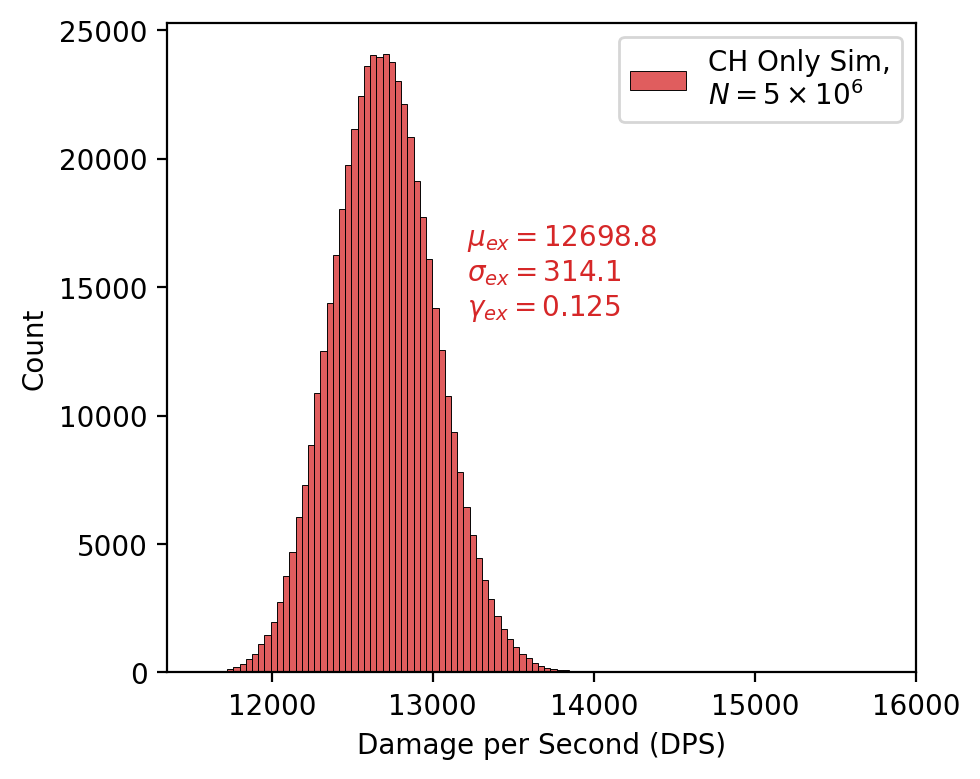
\includegraphics[width=\textwidth]{img/rotation-2-CH.PNG}
            \end{subfigure}
            \hfill
            \begin{subfigure}[b]{0.49\textwidth}
                \centering
                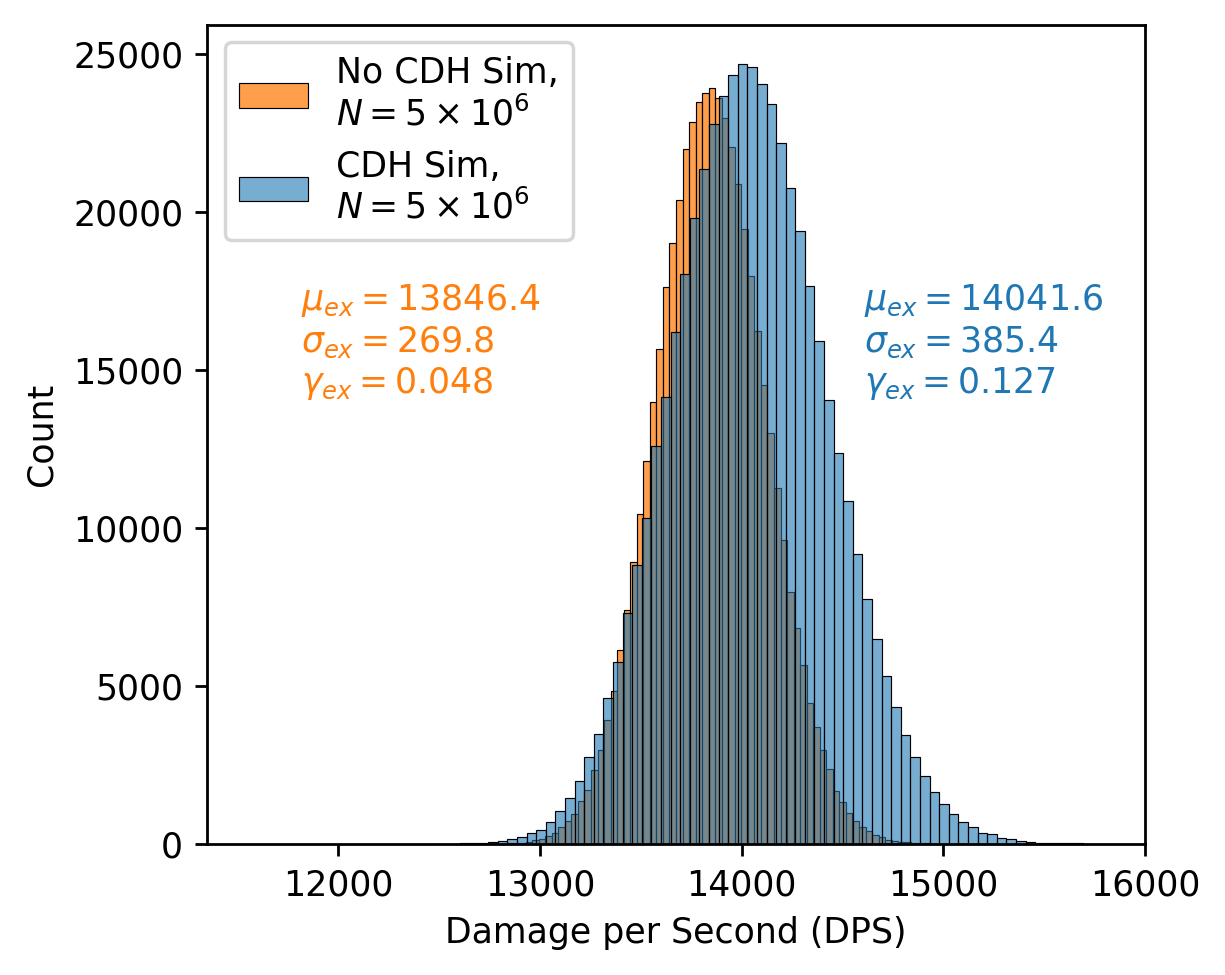
\includegraphics[width=\textwidth]{img/rotation-2.PNG}
            \end{subfigure}
            \caption{Simulated DPS distributions for different hit type combinations for Rotation 2. Each skill is simulated $5 \times 10^6$ times. The exact mean, standard deviation, and skewness for each combination are also shown.}\label{fig:rot-2}
        \end{figure}

        % \begin{figure}[H]
        %     \centering
        %     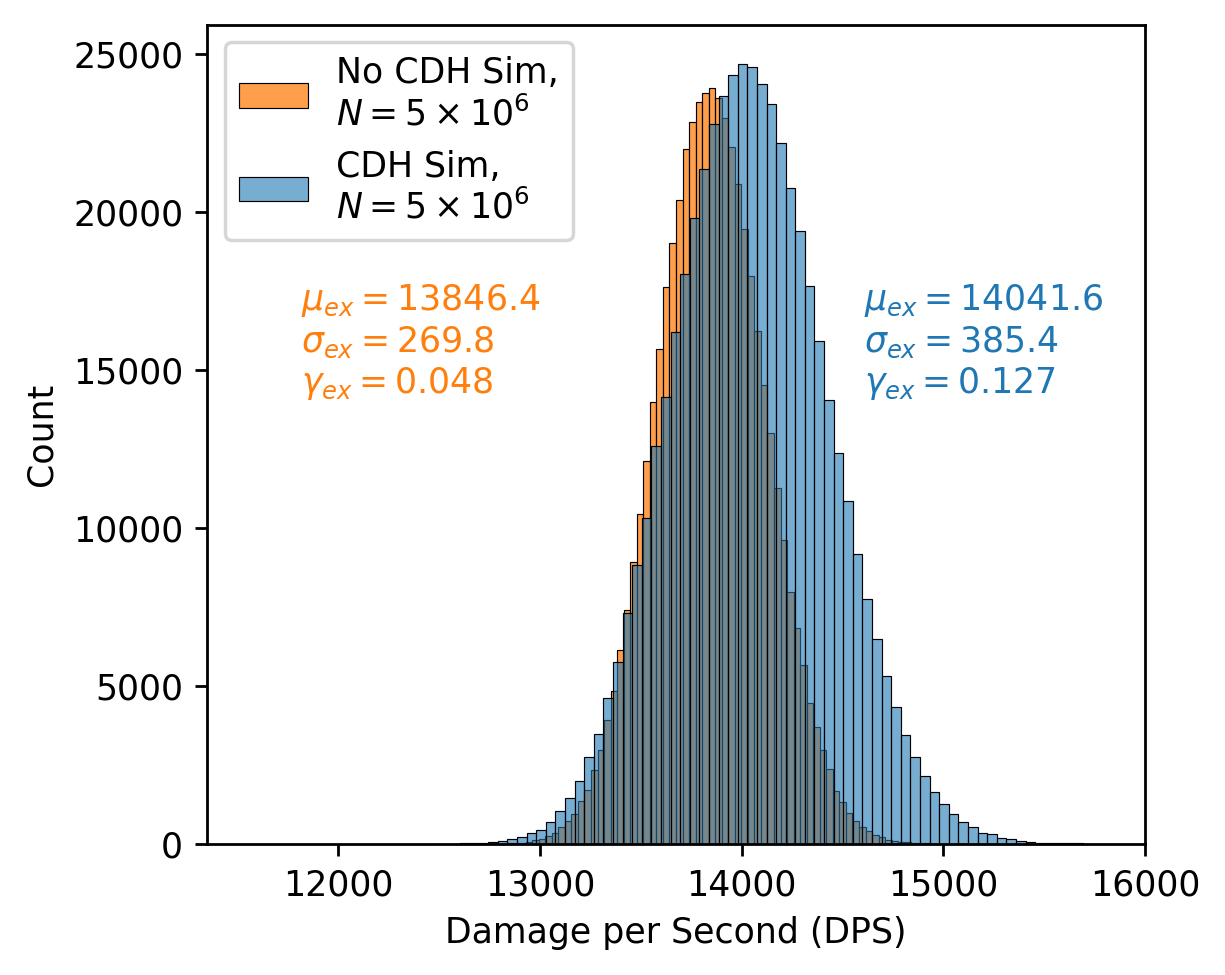
\includegraphics[width=3.5in]{img/rotation-2.PNG}
        % \end{figure}

        The means and standard deviations of Rotation 2 follows a similar trend as Rotation 1 where including additional hit types increases the mean and standard deviation of the DPS distribution. The coefficients of variability also follow a similar trend as in Rotation 1, Table \ref{t:r2-cv}. Allowing direct hits and critical direct hits increases $c_v$ by ca. 11\% more than the standard deviation increased. Removing the possibility of CD hits significantly decreases the coefficient of variation by 21\%. Similarly, excluding CD hits results in a lower skewness, $0.05$, than including CD hits, $0.10$

        \begin{table}[H]
            \centering
            \caption{Coefficient of variation and skewness for different hit-type combinations of Rotation 2. The percent change relative to only normal and critical hits are also shown.}\label{t:r2-cv}
            \begin{tabular}{@{}lllll@{}}
            \toprule
            Hit types present & $c_v$ & \% Change & $\gamma$ & \% Change \\ \midrule
            NH, CH            & 0.025 & 0.0\%     & 0.125    & 0.0\%     \\
            NH, CH, DH        & 0.020 & -21.1\%   & 0.048    & -61.6\%   \\
            All               & 0.027 & 10.9\%    & 0.127    & 1.5\%     \\ \bottomrule
            \end{tabular}
        \end{table}

        \subsection{Discussion}
        A general trend emerges from the two rotations: adding CD hits increases both the variability and positive skewness of a DPS distribution. Both of these trends are undesirable from the perspective of dealing more damage as doing so becomes more reliant on chance than player/party skill.\footnote{It should be stressed that these differences are most important when a rotation is mapped out, optimal, and can be perfectly executed. Changing rotations due to encounter-specific mechanics, using strategies that give more uptime, or just not missing GCDs probably lead to much larger DPS differences than ``bad crit-RNG''. For example, missing one usage of Action 2 and 3 in Rotation 2 causes the average DPS to decrease by ca. 311 DPS, about 1 standard deviation due to hit-type variability.} The exact magnitude of these changes also depends on the the specific critical hit and direct hit rates. The difference in magnitudes is likely because the relationship between the hit-type distribution and damage dealt is non-linear. As the probability a landing a critical hit increases, so to does the damage modifier of a critical hit. Allowing CD hits introduces another non-linear term because the damage modifier is a product of the critical hit and direct hit damage modifiers. To illustrate this relationship with $c_v$, consider a single attack with $D_2 = 10,000$ landing $n = 50$ hits. Figure \ref{fig:ch-dh-scan} shows the exact $c_v$ for all possible critical hit and direct hit rate stat values. Points showing the stat values used for Rotation 1 and Rotation 2 are also shown (note these are not the computed $c_v$ values from the rotations).

        \begin{figure}[H]
            \centering
            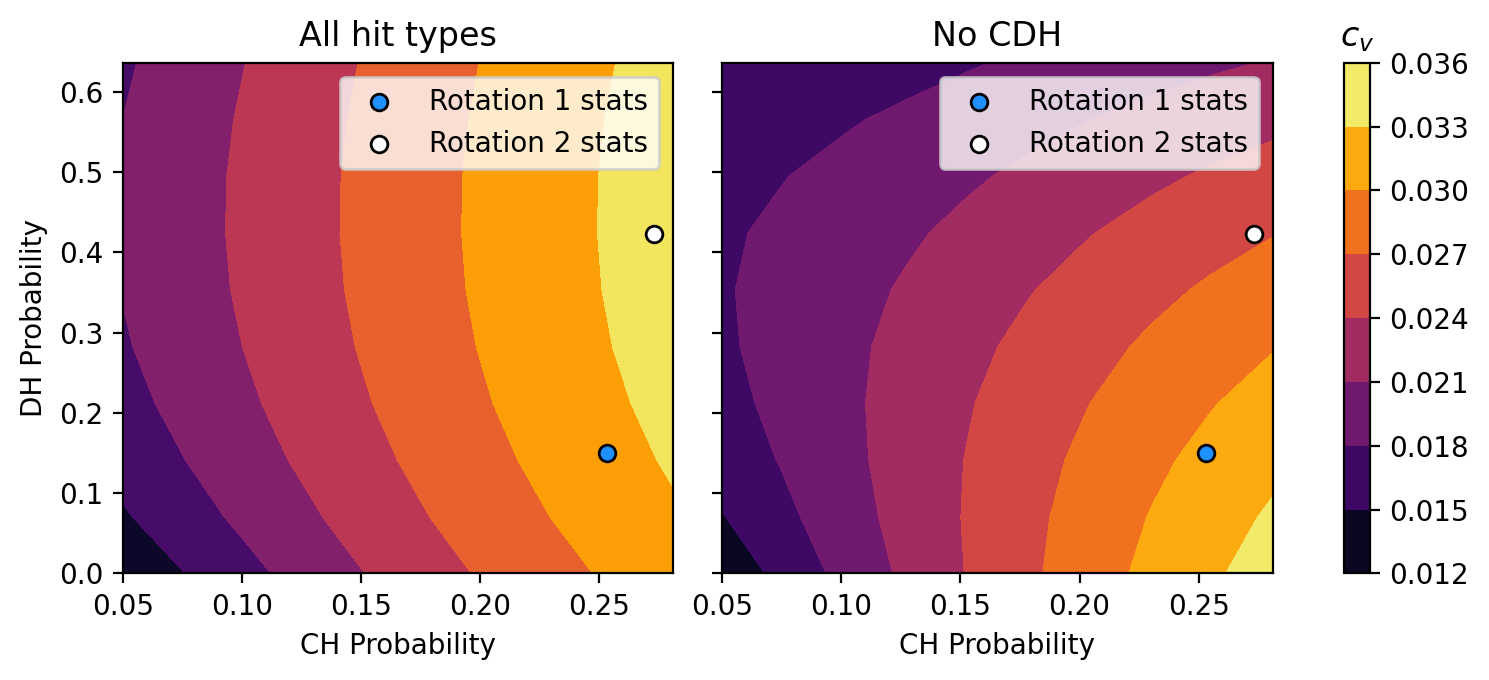
\includegraphics[width=0.9\linewidth]{img/ch-dh-scan.PNG}
            \caption{Contour plot showing $c_v$ for all possible critical hit and direct hit rate stat values for an attack with $D_2 = 10,000$ landing 50 hits. Figure \ref{fig:ch-dh-scan}a (left) includes all possible hit types and Figure \ref{fig:ch-dh-scan}b (right) excludes CD hits. Values along the $x$-axis where DH = $0$ is the case where no direct hits exist.}\label{fig:ch-dh-scan}
        \end{figure}

        Interestingly, the two cases follow different trends. With all hit-types present, both higher direct hit and critical hits rates increase the variability. When CD hits are removed, higher critical hit rates still increases the variability, but a higher direct-hit rate tends to lower the variability. For the stats from Rotation 1, the additional direct hit rate slightly increases $c_v$ relative to DH = $0$. The stats of Rotation 1 are also in a region where removing CD hits mildly changes $c_v$, consistent with the observations in Table \ref{t:r1-cv}. For the stats in Rotation 2, adding direct hit rate also increases $c_v$ relative to DH = $0$ with CD hits. Excluding CD hits, a higher direct hit rate significantly decreases $c_v$ relative to DH $=0$, also consistent with the observations in Table \ref{t:r2-cv}. 
        
        There are probably two factors which influence the variability of the DPS distribution: (i) the damage each hit type deals and (ii) probability of landing each hit type. The variability of the DPS distribution will increase as the damage each hit deals differs more from each other. The critical hit damage from higher critical hit rate amplifies the difference for critical and CD hits with the other hit types, which is probably why higher a higher critical hit rate leads to larger variability for both cases. However, each hit type also must be equally likely as a hit-type that deals significantly different damage but is exceedingly rare will not have a large contribution to metrics that measure variability. A higher critical hit rate and direct hit rate both increases the chance of CD hits, whose damage also differs significantly from the other hit types. If CD hits are excluded, a higher direct hit rate probably decreases the variability because the damage direct hits and critical hits deal are more similar to each other than the damage dealt by normal hits and critical hits. The higher direct hit rate also lowers the chance of landing normal hits.
        A similar scan can also be done for the skewness, Figure \ref{fig:skew-scan}.
        
        \begin{figure}[H]
            \centering
            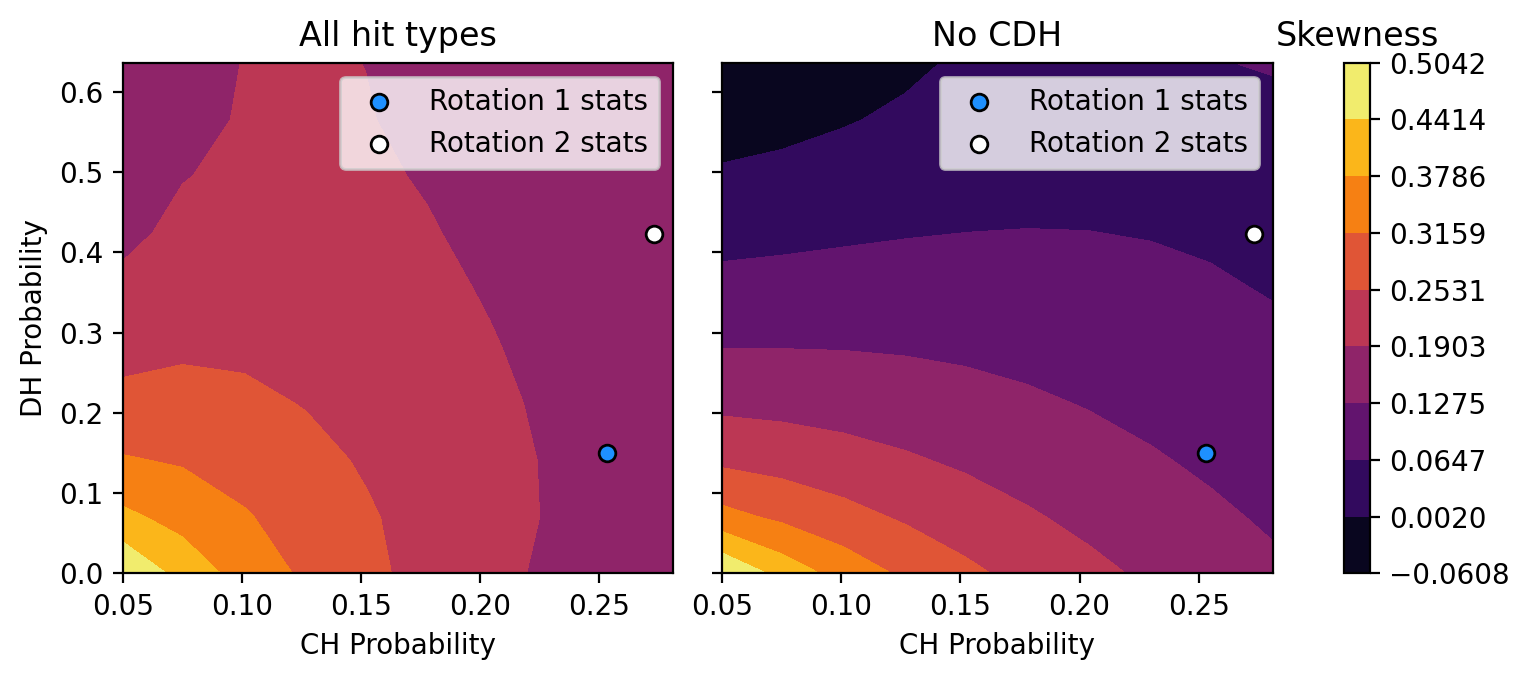
\includegraphics[width=0.9\linewidth]{img/skew-skan.png}
            \caption{Contour plot showing the skewness for all possible critical hit and direct hit rate stat values for an attack with $D_2 = 10,000$ landing 50 hits. Figure \ref{fig:skew-scan}a (left) includes all possible hit types and Figure \ref{fig:skew-scan}b (right) excludes CD hits. Values along the $x$-axis where DH = $0$ is the case where no direct hits exist.}\label{fig:skew-scan}
        \end{figure}

        Increasing both the critical hit rate and direct hit rate decreases the skewness for both cases. However, removing CD hits causes the skewness to decrease more rapidly than when CD hits are present. This seems reasonable, as the binomial (and multinomial) distribution tends towards a normal distribution (where $\gamma = 0$) more quickly when the probabilities are not near 0 or 1. The additional skewness for including all hit types is probably because the damage dealt by CD hits differs more than the other hit types. The other factor which influences how quickly the DPS distribution tends towards a normal distribution is the number of hits. Using the same $D_2 = 10,000$ value, Figure \ref{fig:hit-scan} shows the skewness using the stats from the two rotations, with and without CD hits, for different numbers of hits. 
        
        \begin{figure}[H]
            \centering
            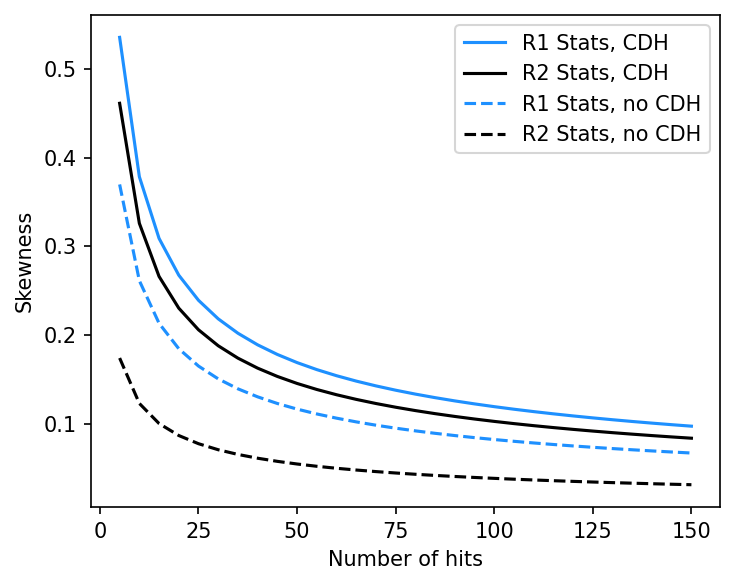
\includegraphics[width=3.3in]{img/hit-scan.png}
            \caption{Skewness at different number of hits for an attack with $D_2 = 10,000$ using the stats of Rotation 1 and Rotation 2. Cases with and without CD hits are shown.}\label{fig:hit-scan}
        \end{figure}

        The skewness for both hit-type combinations decay at similar rates. Removing CD hits lowers skewness, so this case tends towards a normal distribution (which has 0 skewness) more quickly than when CD hits are included. It is also worth reiterating that Figures \ref{fig:ch-dh-scan} - \ref{fig:hit-scan} only shows results for a single hit. Realistic rotations for each job will likely have their own unique, nuanced relationships between the CH/DH rate and the variability of the DPS distribution. Given these results, if the variability and/or the skewness of a DPS distribution wanted to be decreased without outright removing CD hits, one solution could be lowering the chance of a CD hit occuring. Instead of a probability of $p_C p_D$, the probability could be reduced to $\frac{1}{2} p_C p_D$, or by any value from $0-1$. This strategy could similarly be applied to the hit-type damage modifier, \textit{e.g.}, $\frac{1}{2}\lfloor \lfloor \lfloor \lfloor D_2 \lambda_C \rfloor / 1000 \rfloor \lambda_D \rfloor / 100 \rfloor$, or with any value from $0-1$.

        \subsection{Practical aspects}
        To conclude, some of the practical points of modeling a realistic rotation are discussed. The only inputs this framework requires are the probabilities to land each hit type, the damage modifiers from each hit type, which damage buffs are active, and how many total hits are landed. All other stats/traits/etc. enter in as constant parameters. The quantity $D_2$ will depend on Determination, Tenacity, attack power, main attributes, and weapon damage. $D_2$ for auto-attacks and DoT attacks are also affected by Spell/Skill speed and pet damage can also be accounted for since the relevant parameters only affect $D_2$. Additionally, the recast time of the global cooldown depends on Spell/Skill Speed, which affects the conversion factor from total damage dealt to damage per second.
        
        Probably the most difficult aspect of using this framework is correctly counting the number of hits a unique action lands. An action is unique based on its value of $D_2$, $\textbf{p}$, and $\textbf{B}$. Using Dragoon for an example, the number of True Thrust and Vorpal Thrust hits should obviously be counted separately. However, Nastrond, Nastrond with a Lance Charge buff and Nastrond with a Dragon Sight buff should also all be counted separately because the buffs lead to different supports for the damage sub-distributions. The same also applies to skills which affect the rates of hit-types as this alters the weights used to create the mixture distribution in eqn. \ref{eqn:multi-dot-mgf}. Thus, Full Thrust, Full Thrust with Lance Charge, and Full Thrust with Battle Litany should all be counted separately. One important type of action not discussed are those with a random number of hits. Typically, the cooldown timer resets or an action is allowed to be executed based on chance. Writing down the MGFs for skills not tied to the global cooldown, like Bard's Bloodletter, will require selecting the proper support and weights to create the mixture distribution. Actions tied to the global cooldown, like refulgent arrow, are be more complicated because using these skills will affect how many times other actions are used (like burst shot). More work into describing these sorts of actions is certainly needed.

    \newpage
    \newpage

    \section*{Equations for $M^{\prime\prime\prime}_S(t=0)$}
    \begin{figure}[H]
        \centering
        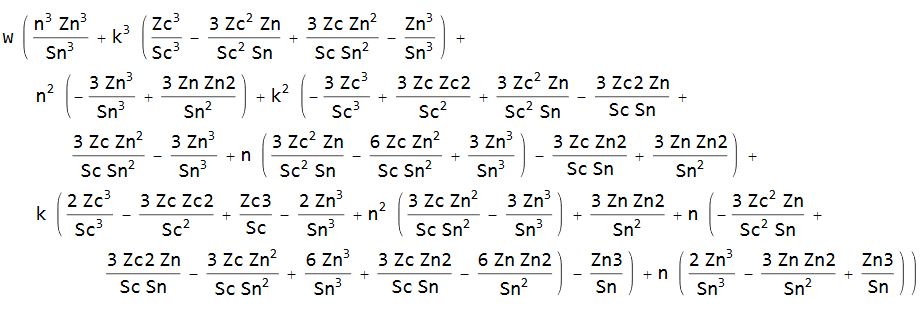
\includegraphics[width=0.85\linewidth]{img/third-deriv-CH.PNG}
        \caption{Expression for $M^{\prime\prime\prime}_S(t=0)$ with $n-k$ normal and $k$ critical hits. Here, $w$ is the corresponding binomial weight given $p_C$.}\label{fig:binom-3rd-deriv}
    \end{figure}

    \begin{figure}[H]
        \centering
        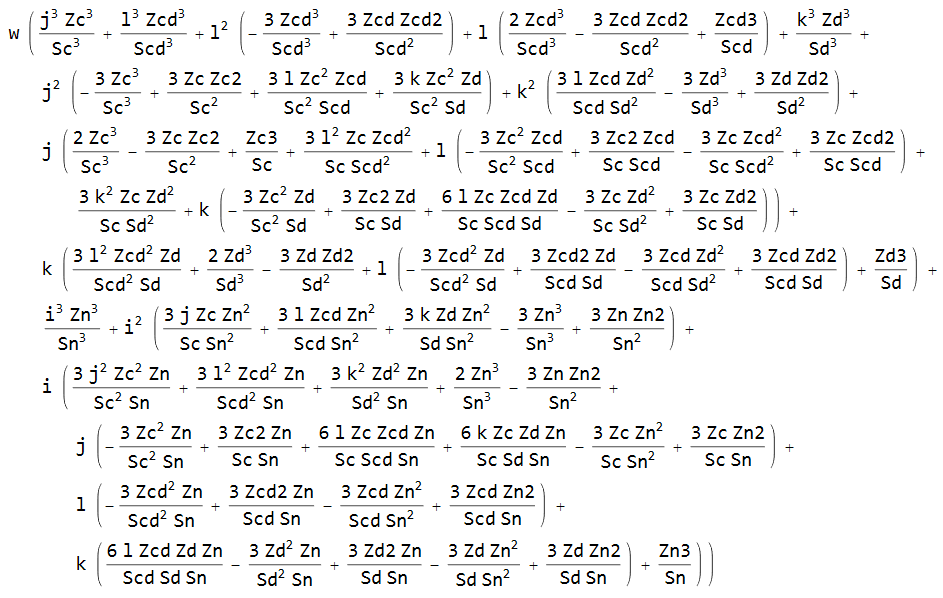
\includegraphics[width=0.9\linewidth]{img/third-deriv.PNG}
        \caption{Expression for $M^{\prime\prime\prime}_S(t=0)$ for $i$ normal, $j$ critical, $k$ direct, and $l$ CD hits. Here, $w$ is the corresponding multinomial weight given \textbf{p}.}\label{fig:multi-3rd-deriv}
    \end{figure}

\end{document}